\section{Maneuver of Interest} \label{sec:maneuver}

To demonstrate CbA, a certification maneuver is needed.
The Generic T-tail Transport, as the name suggests, is based on a commercial transport class aircraft.
It is most closely related to the Bombardier CRJ 700.
A few guiding principals were used in selecting the maneuver of interest:
\begin{itemize}
    \item Real-world certification requirement that the aircraft would be required to pass.
    \item Availability of data required to adequately simulate the maneuver.
    \item Preferably a lateral or directional maneuver that can leverage the multi-dimensional experimental data.
    \item Emphasis on control input to utilize control derivative data.
    \item A quantifiable metric to determine success or failure of the certification maneuver.
\end{itemize}

Based on these guidelines and with the help on industry experts at The Boeing Company, a maneuver was picked from the FAA's \textit{Flight Test Guide for Certification of Transport Category Airplanes} \cite{romanowski_flight_2018}.
Within Chapter \textit{5.3 Directional and Lateral Control} of the guide, the \textit{Lateral Control: Roll Capability \S 25.147(d)} maneuver was chosen.   
The testing procedure is paraphrased as: 
\begin{enumerate}
    \item Airplane starts in a trimmed state for steady straight flight at maximum takeoff speed.
    \item Establish a steady $30^\circ$ banked turn.
    \item Roll the airplane to a $30^\circ$ bank angle in the other direction.
    \item Aircraft must have sufficient roll authority to perform the $60^\circ$ change in bank angle in no more than $11$ seconds. 
    \item The aircraft must be able to do this with one engine inoperative, specifically the one that makes this maneuver more difficult.

\end{enumerate}

Two additional parameters that are mentioned in the guide pertain to the maneuver being unchecked, i.e. roll maneuver doesn't need to stop immediately after the $30 ^\circ$ bank angle is achieved, and that excessive sideslip and bank angle during recovery should be avoided.
Since these are not easily quantifiable parameters, they aren't explicitly enforced in the flight simulation.
With regards to the airplane flap configuration, the guide specifies \textit{"Wing flaps in the most critical takeoff position."}
This is a little vague and while some simulations were run with the flaps deployed at $15^\circ$, in accordance with the CRJ700 Pilot's Handbook, most simulation results that are presented are without flap deflections. 
It was infeasible to run RANS CFD simulations with flaps deployed due to the absence of an accurate geometry with deployed flaps and the significant increase in computational cost that it would merit.  
While engine data is not readily available and, consequently, some modeling was required, the maneuver satisfies all the guiding principals and provides a good platform to showcase the culmination of all the different parts of the work.

A visual representation of the maneuver is shown in Figure \ref{fig:roll_maneuver}. 
For this image, the positive x-axis and the nose of the airplane are pointing out of the page.
For an aircraft that rolls from $\psi = +30^\circ$ to $-30^\circ$ having the right engine be inoperative is the more difficult maneuver.
This is due to the thrust from the operative left engine inducing a yaw moment, and consequently a roll moment, that resists the roll maneuver.
Accordingly, the right engine is labeled as inoperative with the "x" over it.

\begin{figure}
    \center
    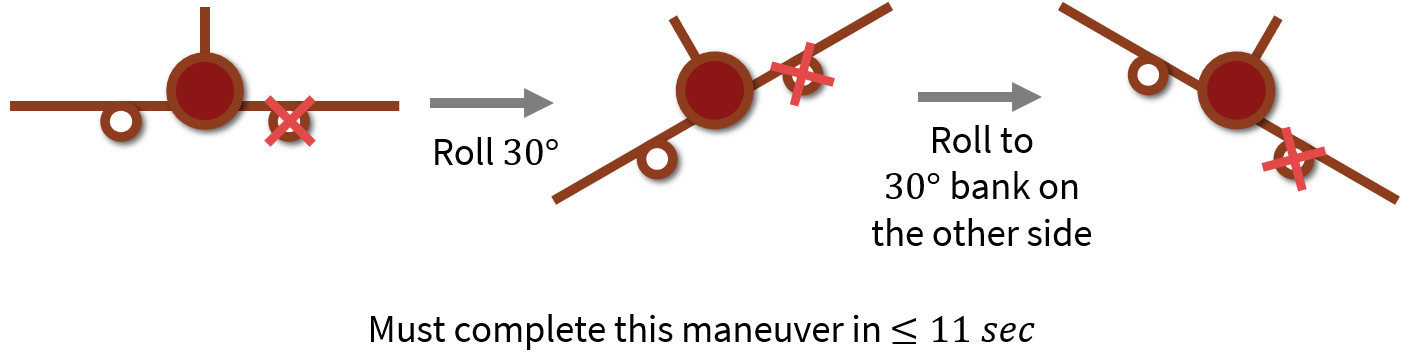
\includegraphics[width=0.95\textwidth]{suthesis/images/roll_maneuver.png}
    \caption{Graphical representation of Roll Capability certification maneuver. \label{fig:roll_maneuver}}
\end{figure}